\chapter{Results}
In this chapter we will present our overall results, by showing our training data, the hyper-parameters used, and
explain what worked and did not work.
Afterwards we will evaluate the best models and present our evaluation data.


\section{Training Experiments}
In \textbf{PPO} there are a number of hyper parameters that can be tweaked to achieve convergence.
An overview of the general parameters used can be seen in Table \ref{tab:hyper}.
\begin{table}[!ht]
    \begin{tabularx}{\linewidth}{lllX}
        \toprule
        Name                       & Value Used       & Method & Description
        \\
        \midrule
        Hands Played & {[}5000,10000,15000{]} & Varied & The number of data points that go into each
        episode. Hands * 4 * 8 \\
        Batch Size                 & 80\% of the data & Fixed  & The absolute size is dependent on the number of
        hands played                 \\
        Epochs & {[}8,12,16{]} & Varied & Number of Epochs per episidode
        \\
        Learning Rate              & 0.0002           & Fixed  & Used for Adams Optimiser
        \\
        Learning Rate Gamma        & 0.3              & Fixed  & Learning rate
        \\
        Clipping Range             & 0.2              & Fixed  & Clipping range to mange the clip the incremental
        change                      \\
        Discount Factor            & 0.99             & Fixed  & Used to calculate Discounted Rewards for
        Non-Terminal steps                  \\
        Value Function Coefficient & 0.5              & Fixed  & (c1) Coefficent that allows computation of a
        comibined loss for actor-critic \\
        Entropy Coefficient        & 0.005            & Fixed  & (c2) Stops the model from early convergence
        \\
        Optimiser Weight Decay     & 1e-5             & Fixed  & Weight decay used in Adams Optimiser
        \\
        \bottomrule
    \end{tabularx}
    \caption{Hyperparameters used throughout the training.}
    \label{tab:hyper}
\end{table}

\subsection{CompleteRL}
For CompleteRL we experimented a fair bit with batch different values of the amount of hands played and it quickly
became apparent that CompleteRL was highly dependent on that number to be large.\\
Anything under 10000 (batch size = 256000,K=16) would simply not converge, and the distribution entropy was hovering
around 0.8, which means that the probabilities of actions effectively represented that of the Random agent.\\
Potential adjustment of the hyper-paramaters might solve this, but we doubt that.
\newline
One experiment that was successful was running 150000 hands(batch size=300000,K=16) over 80 steps.
Fig. \ref{fig:15comp} shows the achieved training progress.
\begin{figure}[!ht]
    \centering
    \subfloat[][Policy Loss]{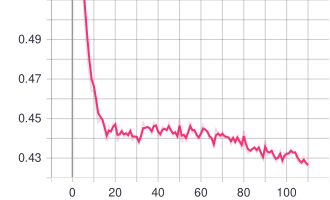
\includegraphics[width=.4\textwidth]{15com/Loss_policy_loss}}\quad
    \subfloat[][Entropy]{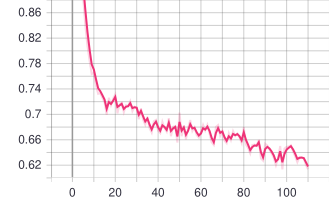
\includegraphics[width=.4\textwidth]{15com/Loss_value_loss}}\\
    \subfloat[][Value Loss]{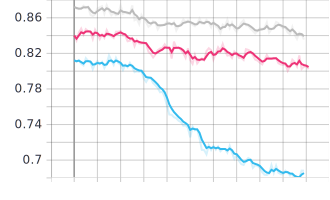
\includegraphics[width=.4\textwidth]{15com/Loss_entropy}}\quad
    \subfloat[][Explained Variance]{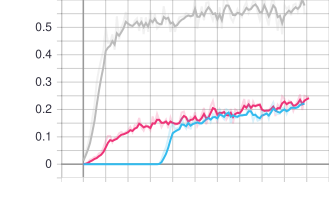
\includegraphics[width=.4\textwidth]{15com/Loss_avg_explained_var}}
    \caption{CompleteRL with 15k and K=16}
    \label{fig:15comp}
\end{figure}

\subsection{SeperatedRL}
For the training of SepereratedRL we experimented with
